\chapter{Test Scenario}
\label{ch:testscenario}
\justifying
\section{Introduction}

This test scenario was designed for newcomers who want to know how to start developing a React Native app. It is based on the Cronometer example developed in PhoneGap from the subject Computación en Red. The app will be developed for Android , and will fearute a very simple cronometer: the user will be able to increase and decrease the amount of time, and start and stop it. The PhoneGap example displays a single view, but this is quite unrealistic, as most current apps have more than one view. Therefore, navigation between views will be added to the example.

The project will be devidided in three stages:

\begin{enumerate}
 \item \textbf{Introduction:} how to create a new project, file system and other important concepts.
 \item \textbf{Creating the first view:} a simple cronometer view will be implemented in this stage step by step.
 \item \textbf{Results:} show the results obtained in the test scenario.
\end{enumerate}

React Native is still a young project in constant development. Currently, installing and getting it to work can be a little tricky, but a good installation guide is available \href{https://facebook.github.io/react-native/docs/getting-started.html}{here}~\cite{rninstallguide}. A very detailed guide has not been included in this work as teaching how to get React Native to work is not its purpose, but instead learning how to develop a hybrid mobile application.

\section{Introduction}

The next tools are necessary to develop an Android app in a Linux environment. Note that how to install them is explained on the tutorial previously mentioned. However, there are a few things missing that on some machines might be required. Because of that, I recommend running the following commands prior to installing anything:

\lstset{style=mybash}
\lstinputlisting[label=rnmissingdeps,language=bash,caption=Missing Guide Dependencies]{./code/rn_missing_dependencies.bash}

\begin{itemize}
  \item \textbf{Required:}
    \begin{itemize}
      \item Git: free and open source distributed version control system. Needed to clone Git projects and to install some of the other tools.~\cite{git}
      \item Node and Node Package Manager (NPM): NPM is a package manager for JavaScript that allows developers to find and share and packages of code.~\cite{node}~\cite{npm}
      \item React Native Command Line Tools (CLI): the React Native CLI allow to create, initialize, update, debug and deploy and application.~\cite{rncli}
      \item Java Development Kit 1.8: React Native requires JDK 1.8 or higher. I recommend the default version from OpenJDK, which can be installed running \code{sudo apt-get install -y default-jdk}.~\cite{jdk}
      \item Android Studio: provides both the Android SDK Tools and an Android emulator (see below). The first ones are needed to compile and generate the android app, while the latter provide a way to quickly see how the mobile app works and feels on a real device.~\cite{androidstudio}
    \end{itemize}

  \item \textbf{Recommended:}
    \begin{itemize}
      \item Watchman: system designed to watch files and record when they change. It can also trigger actions when a change is made.~\cite{watchman}
      \item Flow: static type checker, designed to quickly find errors in JavaScript applications. Current version is 0.27, but React Native uses 0.25. This version mismatch may cause an error, which can be fixed by running \code{npm install -g flow-bin@ReactNativeVersion}. As the current React Native version is 0.25, we would substitute \textit{ReactNativeVersion} with 0.25, but this version is subject to changes as new versions are released.~\cite{flow}
      \item Nuclide: IDE that provides a first-class development environment for writing, running and debugging React Native applications. Currently available for Max and Linux.~\cite{nuclide}
    \end{itemize}
  
  \item \textbf{Emulator:}
    \begin{itemize}
      \item Android Virtual Device (AVD): stock Google Android device emulator that comes with Android Studio. Usually performs well, but can inexplicably fail to run on some systems and sometimes performs badly.~\cite{avd}
      \item Genymotion: altough Android Studio provides a way to emulate a real device, I recommend using Genymotion as it tends to be more stable, runs smoother and is easier to install as well. There are many tutorials for installing it, but I personaly recommend \href{http://techapple.net/2014/07/tutorial-installsetup-genymotion-android-emulator-linux-ubuntulinuxmintfedoraarchlinux/#}{this one}~\cite{genymotioninstall}. Genymotion requires VirtualBox to be installed on your system, so I recommend running this command before: \code{sudo apt-get install -y virtualbox}.~\cite{genymotion}
    \end{itemize}
 

\end{itemize}

\subsection{Creating the project}

The first thing to do is to create a new project. We can do this by opening a terminal, moving to the desired folder and running the following commands:

\lstset{style=mybash}
\lstinputlisting[label=rnprojectfs,caption=React Native project folder,language=bash]{./code/create_project.bash}

This will create a sample project with all the required files and configuration in a folder named \textit{Cronometer}, and move us to the project folder. This folder will contain a series of folders and files very similar to the ones shown in Figure \ref{fig:rnprojectfs}. The whole process might take a few minutes to complete.

\begin{figure}[H]
	\centering
	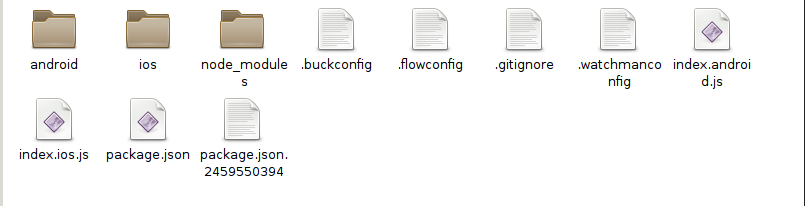
\includegraphics[width=1\linewidth]{rn_project_fs.png}
	\caption{Project folder\label{fig:rnprojectfs}}
\end{figure}

\begin{itemize}
 \item \textbf{Folders}
  \begin{itemize}
   \item android: folder containing the generated code for the Android app. Inside we can find Gradle~\cite{gradle} configuration, Java file sources and the apk generated.
   \item ios: folder containing the generated code for the iOS app. Inside we can find all the necessary information to open the project in XCode~\cite{xcode} and to generate the app.
   \item node\_modules: contains the required node modules, including React Native ones among others.
  \end{itemize}
 \item \textbf{Files}
  \begin{itemize}
   \item index.android.js: main file for the Android app. Here we will start writing our code before spreading it over multiple files as our project grows.
   \item index.ios.js: main file for the iOS app. In this project this file will be left unmodified because it is not required for the Android app.
   \item package.json: file containing vital information about the project like the own project name, dependencies, versions, and a long etc. Current dependencies are \code{react} and \code{react-native}, but if we want to add new modules and automatically include them in this file, we should add the \code{--save} option when running a \code{npm install} command. For this project, hoewever, the two dependencies mentioned will suffice as they provide all the core components and functionalities for a mobile application.
  \end{itemize}
\end{itemize}

\subsection{Running the app for the first time on the emulator}

To check that the project we just created runs fine and mistakes were made, we are going to try it out on the Android device emulator. Run your device, either from the Android Virtual Device window or from Genymotion. Once the emulator has finished loading, it is time to try our app. Open two more terminals and navigate to the project folder in both of them. Type the following:

\begin{description}
 \item First Terminal: \code{react-native start}.
 \item Second Terminal: \code{react-native run-android}
\end{description}

On the first terminal we start the packager, which bundles the whole application as a single JavaScript file and delivers it when receiving a GET request on port 8081. We can take a look at the bundle by typing \url{http://localhost:8081/index.android.bundle} on the browser. The second one tells React Native to run the Android version of our project. It automatically installs the application on the virtual device, which requests the bundle. If everything is ok, one should see something similar to what is shown on Figure \ref{fig:rnemulator1}.

\begin{figure}[H]
	\centering
	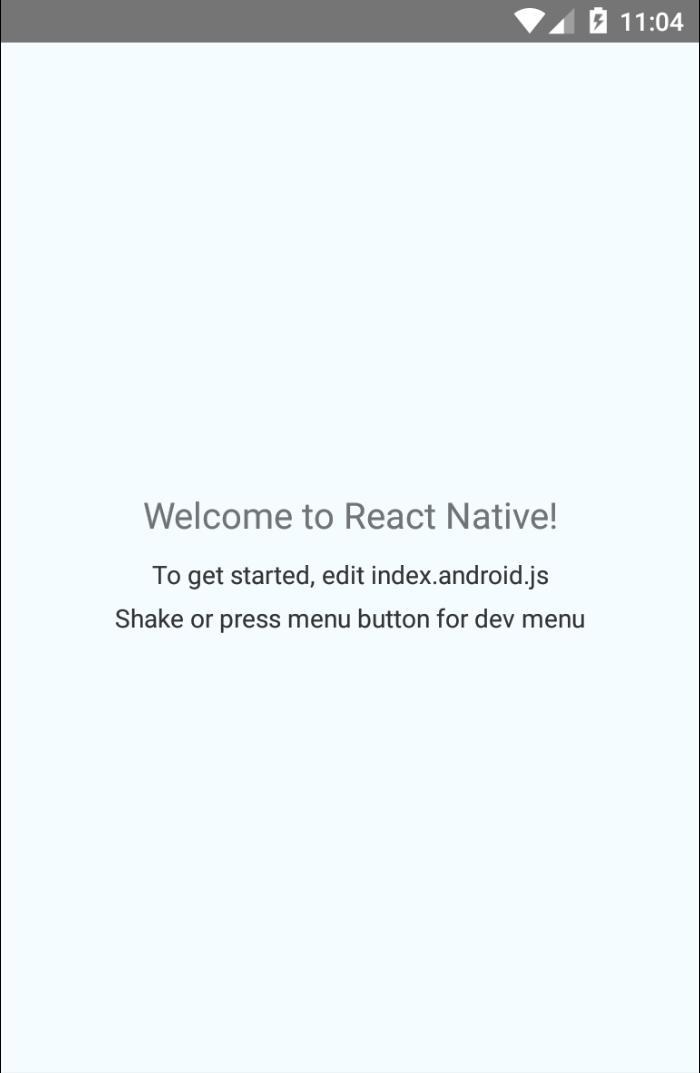
\includegraphics[width=0.5\linewidth]{rn_emulator_1.png}
	\caption{First view of the app\label{fig:rnemulator1}}
\end{figure}

To open de developer tools in the emulator, simply press Control + M on Linux or Control + \cmdkey + Z on Mac. However, the key-bindings may vary between systems, so for more information click \href{https://facebook.github.io/react-native/docs/debugging.html}{here}~\cite{opendevtools}.

\section{Creating the first view}

In this work, Nuclide was used as the IDE, but any text editor will do the trick. However, using Nuclide is highly recommended since it was designed for developing React Native apps and enables many features like Flow that otehrwise would be useless. Flow provides type checking, which is helps avoiding errors and other nuisances. It also allows tabbing differente files, global searches and working on a remote server, among other features.

In case we are using Nuclide, open it and click on \textit{Add Project Folder}, add our project folder and double click on the file \textit{index.android.js}. The code we can see is the default application that React Native creates when Initializing a project. As we can see, the structure is the same as the described on Paragraph \ref{subsec:nativecomps}. There are a few imports, a single class which comprises the whole view shown in Figure \ref{fig:rnemulator1} and some styling.

Before running around like a headless chicken, it is highly recommended to spend a few minutes thinking about what are we going to do and how. For this purpose, we can use a very simple class diagram, based on the Unified Modeling Language (UML)~\cite{uml}~\cite{umlbook}.

\begin{figure}[H]
	\centering
	\includegraphics[width=0.25\linewidth]{1_class_diagram.png}
	\caption{First class diagram\label{fig:1rnclassdiagram}}
\end{figure}

As we can see in Figure \ref{fig:1rnclassdiagram}, we will only need one class, named \textit{Cronometer}. This class will have two attributes and five methods, which names are self-explanatory. However, when working with React Native and mobile applications, we must also think about the user interface and how the user will interact with out application. A quick example: if we want to start and stop the cronometer, we could place two buttons, one to start it and one to stop it; but we could also use the same button for both actions, depending on the current state of the cronometer. This way, when the cronometer is not running, the button could read \textit{Play}, and once the user pressed it and the cronometer would start running, the text could switch to \textit{Stop}, and vice versa.

To implement a cronometer, we will need some kind of timer to measure seconds. React Native does include some very basic and low-level timing functions, but are hard to use and tend to cause trouble. For this reason, we are going to make use of a module available through NPM. To install it, open a terminal, navigate to the project folder and type \code{npm install --save react-native-timer}. This will install the package and directly save it into the \textit{package.json} as a dependency.

Now, lets get out hands dirty and start modifying our app. Except otherwise stated, we will only modify the \textit{index.android.js}. Firstly, we will modify the imports to include a few new components and the timer module we downloaded. Logically, using a module which has not been imported will crash the app. The resulting code is shown on Figure \ref{lst:1imports}.

\lstset{style=myhtml}
\lstinputlisting[label={lst:1imports},caption=Imports,language=JavaScript]{./code/1.index.android.js}

Now, lets move to the core class of our app. Our \textit{Cronometer} class extends the \textit{Component} class from React, so we can use all the methods inherited such as the lifecycle methods explained on Chapter \ref{ch:reactnative} and the \code{render()} method, and add our own to the app's logic.

\lstset{style=myhtml}
\lstinputlisting[label={lst:1imports},caption=Application's logic summary,language=JavaScript,linewidth=15cm]{./code/2.index.android.js}

Our app will have nine methods which are described next.

\subsection{constructor(props) and componentDidMount()}

\lstset{style=myhtml}
\lstinputlisting[label={lst:1methods1},caption=constructor(props) and componentDidMount(),language=JavaScript]{./code/1.constructor.js}

React Native uses the ES6 class syntax~\cite{es6} along with an API very simmilar to \code{React.createClass}. However, nstead of providing a separate \code{getInitialState} method, you set up your own state property in the constructor. \code{propsTypes} and \code{defaultProps} are defined as properties on the constructor as well. 

Invoking \code{super(props)} is mandatory in the constructor so the props are properly set. After that, we set the state with 6 variables:

\begin{itemize}
 \item play: boolean, records if the cronometer's state: \code{false} means it is stopped, while \code{true} means it is running.
 \item time: records the amount of seconds left.
 \item x, y, w, h: x coordinate, y coordinate, width and height respectively. React Native uses flexbox, among other polyfills, to create adaptable user interfaces that keep their proportions independently from the device screen size (see Paragraph \ref{subsec:stlyes}). This variables will be used to store the clock sphere image position and size, se we are able to place the clockhand right in the middle.
\end{itemize}

The \code{componentDidMount()} method will be executed once, right after the component is mount. Its only purpose is calling the method \code{measureCronoImage()}, which will be explained next. However, this method is called from a \code{setTimer()}. At first glance, this may seem weird, but lets recall the component initialization in React (see Figure \ref{fig:rncomplifescenarios}). We cannot measure a component that has not been already rendered, and this is done almost at the end, right before the \code{componentDidMount()} method. Ok, so we measure it after the user interface has been rendered. However, this leaves us with no clockhand at all until teh state changes, because all the state variables were assigned a value of 0, and no additional render is triggered in \code{componentDidMount()}. Therefore, we need to set a timer that calls the \code{measureCronoImage()} method right after the component initialization has finished, so it triggers another render and we can see the clockhand from the beggining.

\subsection{measureCronoImage()}

\lstset{style=myhtml}
\lstinputlisting[label={lst:1methods2},caption=measureCronoImage(),language=JavaScript]{./code/1.measureCronoImage.js}

This method measures the view contaning the clock sphere and updates the state variables, therefore triggering an update. The view is accessed through a reference set in the \code{render()} method (see Paragraph \ref{subsec:render}), and the \code{measureInWindow()} method is inherited from the Component class. It is important to note that axis coordinates in React Native work like is shown in Figure \ref{fig:rnaxis}. It is also important to remmeber that, when giving a view absolute coordinates, these are relative to the parent view, and not to the root layout.

\begin{figure}[H]
	\centering
	\includegraphics[width=0.3\linewidth]{rn_axis.png}
	\caption{Coordinate axis in React Native\label{fig:rnaxis}}
\end{figure}

\subsection{onSubtractPressed() and onAddPressed()}

\lstset{style=myhtml}
\lstinputlisting[label={lst:1methods3},caption=onSubtractPressed() and onAddPressed(),language=JavaScript]{./code/1.onSubtractPressed.js}

\code{onSubtractPressed()} will be called when the subtract button is pressed, while \code{onAddPressed()} does the opposite. Each time one of them is called, they modify \code{this.state.time} and an update is triggered, rendering the view again and displaying the changes.

\subsection{onNextOpButtonPressed()}
\label{subsec:onnextopbuttonpressed}

\lstset{style=myhtml}
\lstinputlisting[label={lst:1methods4},caption=onNextOpButtonPressed(),language=JavaScript]{./code/1.onNextOpButtonPressed.js}

This method starts or stops the cronometer depending on the current state. The methods in charge of doing it are described in the next paragraph. In case that time left has already reached 0, it does nothing; otherwise, it simply negates the current value of \code{this.state.play} and calls the appropirate method.

\subsection{startCrono() and stopCrono()}

\lstset{style=myhtml}
\lstinputlisting[label={lst:1methods5},caption=startCrono() and stopCrono(),language=JavaScript]{./code/1.startCrono.js}

\code{startCrono()} sets and interval which decreases the amount of time left by 1 second and checks if the amount if time left is 0. In that case, it shows an alert and stops the cronometer.

\code{stopCrono()} is a very simple method as it only clears the timer, therefore stopping the cronometer.

\subsection{render()}
\label{subsec:render}

\lstset{style=myhtml}
\lstinputlisting[label={lst:1methods6},caption=render(),language=JavaScript]{./code/1.render.js}

In the render method is where the user interface is implemented. It is by far the largest method, and so it was split in sections using comments. React Native uses nested components and JSX syntax, so you just need to put \code{\{ \}} around a comment when you are within the children section of a tag.

\begin{description}
 \item \textbf{Preparation and container:} \code{this.state.time} is read. The only view in this fragment is the root parent View, which fills the screen and contains all of the other elements of the user interface. Following views will be placed by default one below another, filling the space specified in the StyleSheet descibed in Paragraph \ref{subsec:styles}.
 \item \textbf{Title:} a single View containing a Text. 
 \item \textbf{Add and subtract buttons:} another View contains three elements: two TouchableOpacity elements and one Text. The simplest one is, of course, the Text, which displays the value of the variable created  at the beggining of the method and contains the time remaining. In this case, the parent \code{style} has been defined to place its elements in a row, instead of a column. There are four kinds of elements for making views respond properly to touches, but it is highly recommended to stick with two first ones.
 
 \begin{itemize}
   \item TouchableOpacity: on press down, the opacity of the wrapped view is decreased, dimming it. This is done without actually changing the view hierarchy, and in general is easy to add to an app without weird side-effects. Should be the first choice when implementing a touch-sensitive view.
   \item TouchableHighlight: on press down, the opacity of the wrapped view is decreased, which allows the underlay color to show through. This is done by adding a view to the view hierarchy, which can sometimes cause unwanted results if not used correctly.
   \item TouchableNativeFeedback: similar to the previous ones, but uses native state drawable to display touch feedback. Should only be used when there are no alternatives.
   \item TouchableWithoutFeedback: provides touch responsiveness without visual feedback, which is why using it is strongy discouraged.
  \end{itemize}

 In this case, the first TouchableOpacity element is the subtract button, and calls the \code{onSubtractPressed()} method when pressed; while the second TouchableOpacity element is the add button, which calls the \code{onAddPressed()} method. Inside each of them there is a Text element with a plus or minus symbol.
 
 As a side note, simply pointing out that these four elements onyl support a single child view.
  
 \item \textbf{Clock sphere:} this fragments contains a single View and an Image element which fills the whole view. A reference has been created to make the it visible to the rest of the class and be able to measure it in the \code{measureCronoImage} method. The Image source can come from the hybrid app's resources or from the network. In this case we are working with an image from the resources, as we can see in the line \code{source={require(`./img/crono.png')}}. To load a network image, is as simple as using a URI, e.g \code{source=\{\{uri:`https://goleta.etsit.}
 \code{upm.es/actas/images/escudos/logoescuela.jpg'\}\}}
 
 \item \textbf{Clockhand container:} parent view for the clockhand. In this case, the positiong is absolute to the parent view, which in this case is the root layout view as well. Its style has been directly defined because it depends on the current state. This view contains two more, the clockhand and the red tip, so when we rotate the parent view within the \code{transform} section, the whole view will rotate as if it was a single one. This saves us from the task of calculating the right position for both of the children views and rotating them independently.
 \item \textbf{Clockhand:} made of two different views: the clockhand itself is the first one, while the latter will render the red tip. Again, like their parent view, their positioning is absolute, but in this case it is absolute to their parent view, instead of the root layout view.
 \item \textbf{Start/stop button:} finally, another view contains the TouchableOpacity element that acts as the Start/Stop button. When pressed, it will trigger the \code{onNextOpButtonPressed()} method that was detailed on Paragraph \ref{subsec:onnextopbuttonpressed}. The source image depends on the current state of the cronomenter.
\end{description}

\subsection{Styles}
\label{subsec:styles}

\begingroup
\lstset{style=myhtml,linewidth=7cm}
\captionsetup{labelformat=empty,labelsep=none}
\lstinputlisting[label={lst:1styles},language=JavaScript,multicols=2,title=]{./code/1.styles.js}
\endgroup
\begingroup
\captionof{lstlisting}{Application's StyleSheet.}
\endgroup

On Listing \ref{lst:1styles} the styles that each user interface view will adopt are specified. Some of those tags are common with HTML, but some others like \code{flex} or \code{flexDirection} will not. Therefore I will not go into detail with most of the attributes, but instead will describe some of the polyfills that React Native uses.

A polyfill is a piece of code that implements a feature that is not supported. React Native uses them to implement features that are available for web development. These libraries can be installed using \code{npm install}. Current imlemented polyfills are the following:

\begin{itemize}
 \item \textbf{Flexbox:} by far the most useful and used, 100\% apps written in React Native use it. Flexboxmodule (currently a W3C Last Call Working Draft) aims at providing a more efficient way to lay out, align and distribute space among items in a container, even when their size is unknown and/or dynamic.~\cite{flexbox}

 The main idea behind the flex layout is to give the container the ability to alter its items' width/height (and order) to best fill the available space (mostly to accommodate to all kind of display devices and screen sizes). A flex container expands items to fill available free space, or shrinks them to prevent overflow.

 Flexbox properties are separated in two categories, depending on the type of element: parent properties and children properties. Obviously, the parent or flex container contains children or flex items. Some of the most importante properties are:

 \begin{itemize}
  \item flex-direction (parent): establishes the main axis, defining the direction that flex items will be placed in the flex container.
  \item justify-content (parent): defines the alignment along the main axis, be it in the left, center, right, equally spaced...
  \item align-items (parent): defines the default behaviour for how flex items are laid out along the cross axis on the current line.
  \item align-content (parent): aligns a flex container's lines within when there is extra space in the cross-axis.
  \item align-self (child): this allows the specified alignment to be overridden for individual flex items.
 \end{itemize}

 \item \textbf{ShadowPropTypesIOS:} enables the UIView shadow properties.
 \item \textbf{Geolocation:} available for Android and iOS. Enables the use of native geolocation functions.
 \item \textbf{Network:} one of the most important APIs. It supports REST requests,  full-duplex communication over TCP and an XML request method.
 \item \textbf{Timers:} this API has already been used in this project, so there is not much more to say. Aside from the timers, it also implements an \code{InteractionManager} which can be used to schedule expensive operations and avoid delaying active animations.
 \item \textbf{Colors:} quite self-explanatory, it enables a dozen commands for color declaration and over a hundred pre-made colors.\cite{ftt2011}
\end{itemize}

\section{Results}

A simple mobile application has been developed using React Native. All the code has been uploaded to a GitHub repository and is available for download \href{https://github.com/IgnacioMV/Cronometer}{here}~\cite{repo}.The source images can be found in the folder \textit{img} inside the project. The results should be the following:

\begin{figure}[H]
\centering
\begin{minipage}{.5\textwidth}
  \centering
  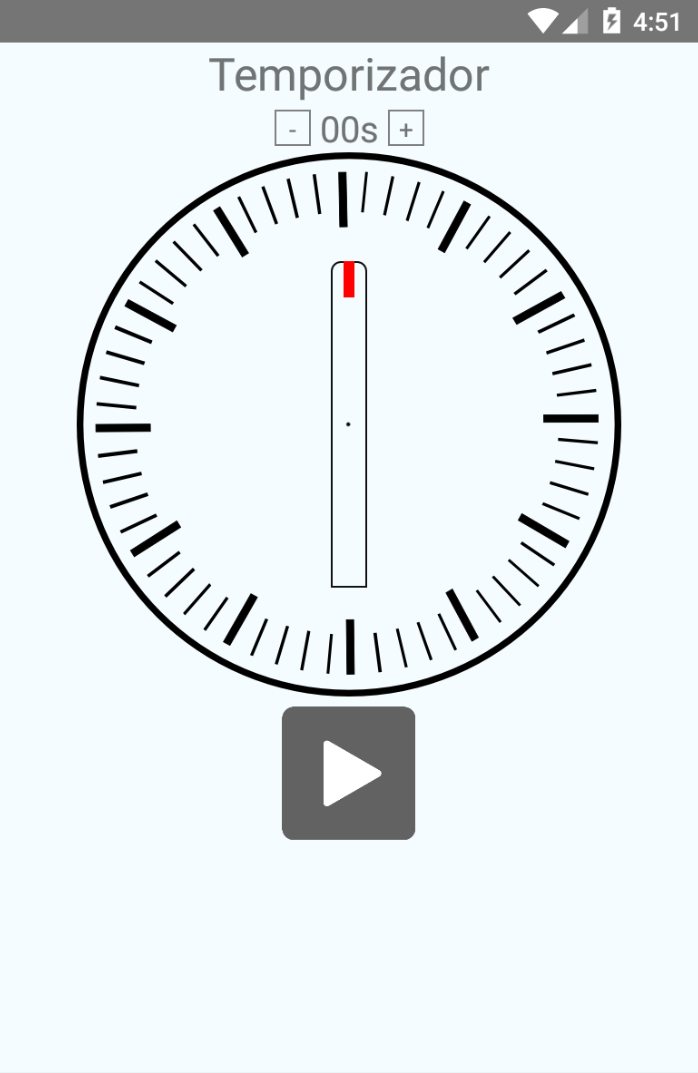
\includegraphics[width=0.8\linewidth]{rn_crono_stopped.png}
  \caption{Cronometer stopped\label{fig:rncronostoppd}}
  \label{fig:test1}
\end{minipage}%
\begin{minipage}{.5\textwidth}
  \centering
  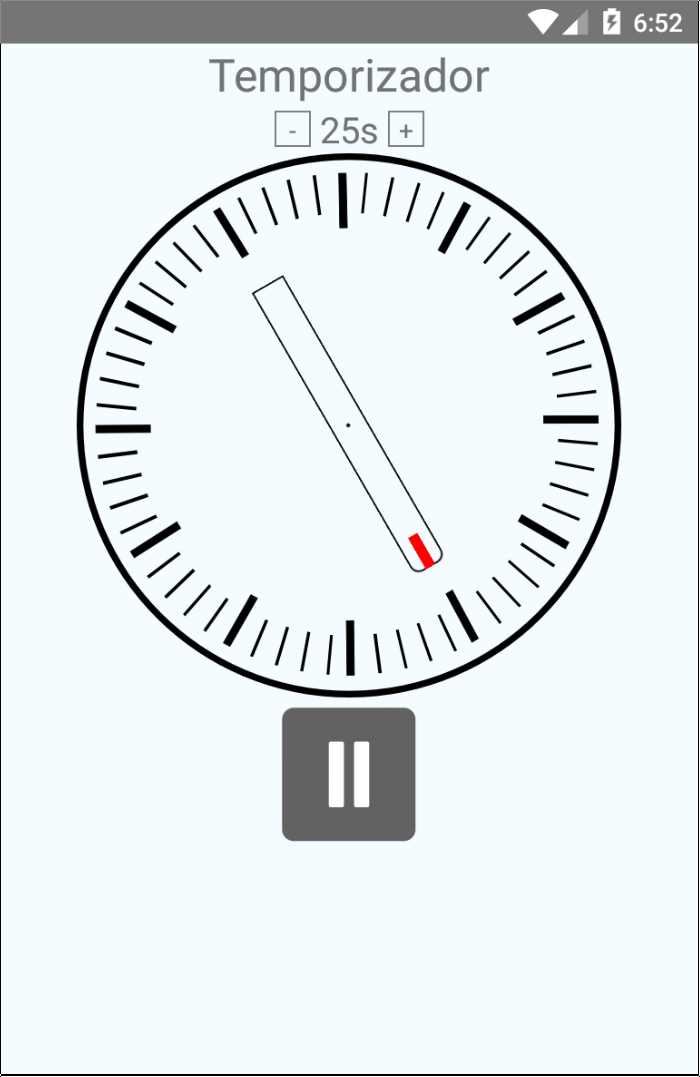
\includegraphics[width=.8\linewidth]{rn_crono_running.png}
  \caption{Cronometer running\label{fig:rncronorunning}}
  \label{fig:test2}
\end{minipage}
\end{figure}

When the user presses de + button, the clockhand will rotate clockwise, and vice versa when the user presses the - button. Clicking on the play button will start the crono, and clicking again will stop it.